RGG installers can be obtained at \url{http://cmb.kitware.com/CMB/resources/software.html} for all three major operating systems: Windows, Mac OS X, and Linux.  Detailed installation guides are detailed below by platform.

\section{Windows}
A security warning may come up and ask for permission to allow the installer to make changes to your computer.  Be sure to click \emph{Yes} to allow the installation process to continue.  This may require authentication by your computer's administrator.

A window like the one shown below should come up.

\begin{figure}[H]
	\begin{center}
		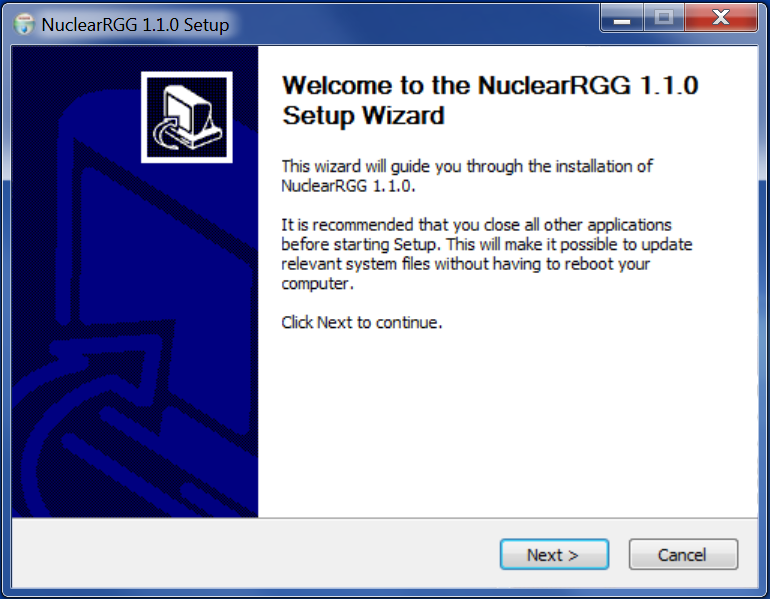
\includegraphics[width=0.5\linewidth]{Images/windows-install-1.png}
		\caption{Beginning the installation process.}
		\label{fig:WindowsInstall1}
	\end{center}
\end{figure}

Click \emph{Next} to continue and agree to the license displayed.  On the next screen (shown below), either use the default install location or select one of your own.  Click \emph{Next}.

\begin{figure}[H]
	\begin{center}
		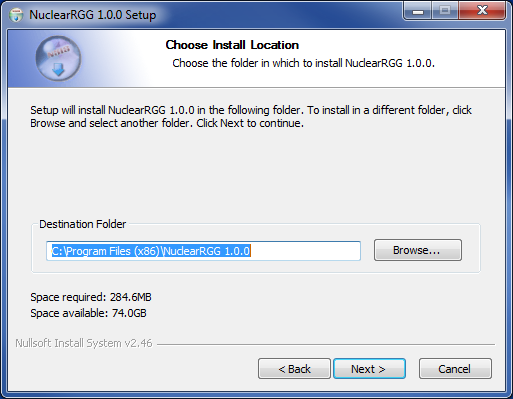
\includegraphics[width=0.5\linewidth]{Images/windows-install-2.png}
		\caption{Selecting the install location.}
		\label{fig:WindowsInstall2}
	\end{center}
\end{figure}

On the next window (shown below), select whether or not you'd like a Start Menu Folder to be created for RGG.  If you would not link a Start Menu Folder to be created, select the \emph{Do not create shortcuts} box.  Otherwise, confirm the Start Menu Folder name you'd like to use.  Click install to have the installer extract the binaries.

\begin{figure}[H]
	\begin{center}
		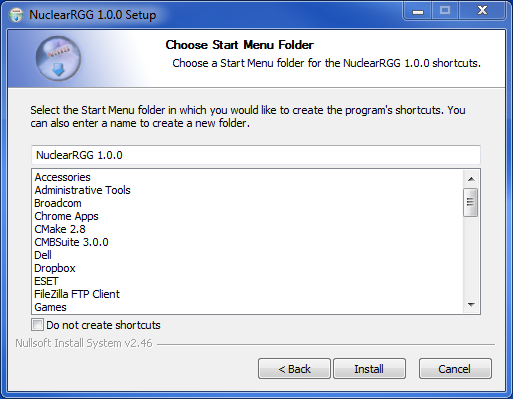
\includegraphics[width=0.5\linewidth]{Images/windows-install-3.png}
		\caption{Configuring Start Menu Folders.}
		\label{fig:WindowsInstall3}
	\end{center}
\end{figure}

A window should come up to confirm that RGG has been sucessfully installed on your computer.  At this point, you can click \emph{Finish} to close this wizard.

\section{Mac}
We use a standard drag and drop installer on Mac.  Simply mount the .dmg file and drag the RGG app into the Applications folder alias.

\section{Linux}
\todo{Figure out what CPack Generator we use for Linux packages.  Will we distribute a .deb, .rpm, or only tarballs and zip archives?}